% Created by tikzDevice version 0.12.3 on 2020-04-17 11:56:46
% !TEX encoding = UTF-8 Unicode
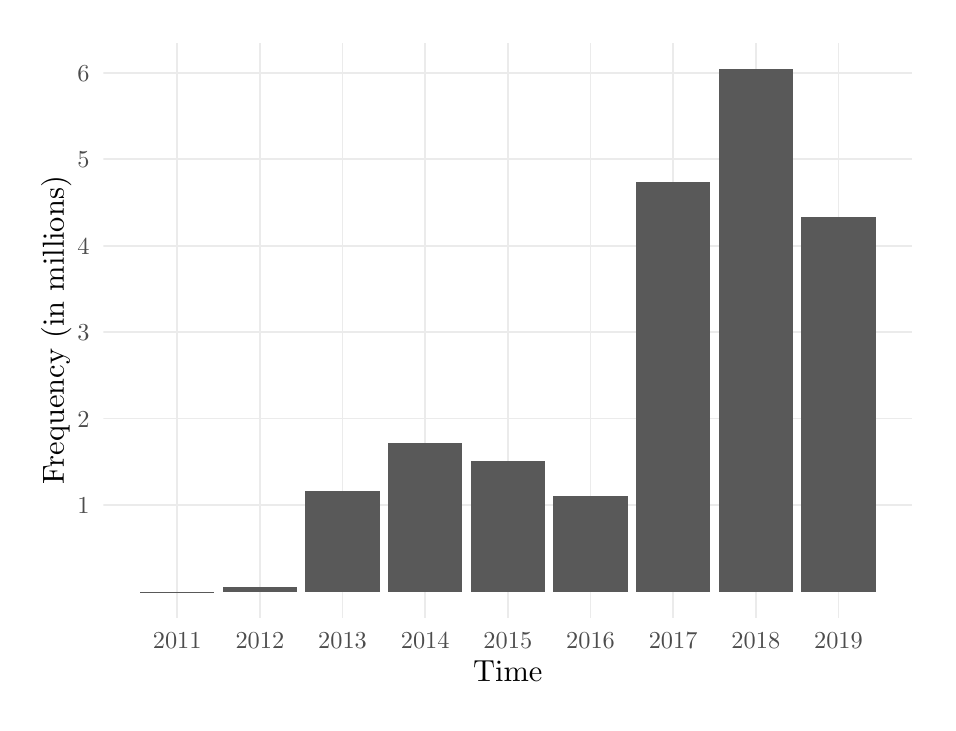
\begin{tikzpicture}[x=1pt,y=1pt]
\definecolor{fillColor}{RGB}{255,255,255}
\path[use as bounding box,fill=fillColor,fill opacity=0.00] (0,0) rectangle (325.21,243.91);
\begin{scope}
\path[clip] ( 27.31, 30.69) rectangle (319.71,238.41);
\definecolor{drawColor}{gray}{0.92}

\path[draw=drawColor,line width= 0.6pt,line join=round] ( 27.31, 71.38) --
	(319.71, 71.38);

\path[draw=drawColor,line width= 0.6pt,line join=round] ( 27.31,102.63) --
	(319.71,102.63);

\path[draw=drawColor,line width= 0.6pt,line join=round] ( 27.31,133.88) --
	(319.71,133.88);

\path[draw=drawColor,line width= 0.6pt,line join=round] ( 27.31,165.13) --
	(319.71,165.13);

\path[draw=drawColor,line width= 0.6pt,line join=round] ( 27.31,196.38) --
	(319.71,196.38);

\path[draw=drawColor,line width= 0.6pt,line join=round] ( 27.31,227.63) --
	(319.71,227.63);

\path[draw=drawColor,line width= 0.6pt,line join=round] ( 54.04, 30.69) --
	( 54.04,238.41);

\path[draw=drawColor,line width= 0.6pt,line join=round] ( 83.91, 30.69) --
	( 83.91,238.41);

\path[draw=drawColor,line width= 0.6pt,line join=round] (113.78, 30.69) --
	(113.78,238.41);

\path[draw=drawColor,line width= 0.6pt,line join=round] (143.65, 30.69) --
	(143.65,238.41);

\path[draw=drawColor,line width= 0.6pt,line join=round] (173.51, 30.69) --
	(173.51,238.41);

\path[draw=drawColor,line width= 0.6pt,line join=round] (203.38, 30.69) --
	(203.38,238.41);

\path[draw=drawColor,line width= 0.6pt,line join=round] (233.25, 30.69) --
	(233.25,238.41);

\path[draw=drawColor,line width= 0.6pt,line join=round] (263.12, 30.69) --
	(263.12,238.41);

\path[draw=drawColor,line width= 0.6pt,line join=round] (292.98, 30.69) --
	(292.98,238.41);
\definecolor{fillColor}{gray}{0.35}

\path[fill=fillColor] ( 40.60, 40.13) rectangle ( 67.48, 40.14);

\path[fill=fillColor] ( 70.47, 40.13) rectangle ( 97.35, 41.72);

\path[fill=fillColor] (100.34, 40.13) rectangle (127.22, 76.56);

\path[fill=fillColor] (130.21, 40.13) rectangle (157.09, 93.65);

\path[fill=fillColor] (160.07, 40.13) rectangle (186.95, 87.49);

\path[fill=fillColor] (189.94, 40.13) rectangle (216.82, 74.68);

\path[fill=fillColor] (219.81, 40.13) rectangle (246.69,188.20);

\path[fill=fillColor] (249.68, 40.13) rectangle (276.56,228.97);

\path[fill=fillColor] (279.54, 40.13) rectangle (306.42,175.66);
\end{scope}
\begin{scope}
\path[clip] (  0.00,  0.00) rectangle (325.21,243.91);
\definecolor{drawColor}{gray}{0.30}

\node[text=drawColor,anchor=base east,inner sep=0pt, outer sep=0pt, scale=  0.88] at ( 22.36, 68.35) {1};

\node[text=drawColor,anchor=base east,inner sep=0pt, outer sep=0pt, scale=  0.88] at ( 22.36, 99.60) {2};

\node[text=drawColor,anchor=base east,inner sep=0pt, outer sep=0pt, scale=  0.88] at ( 22.36,130.85) {3};

\node[text=drawColor,anchor=base east,inner sep=0pt, outer sep=0pt, scale=  0.88] at ( 22.36,162.10) {4};

\node[text=drawColor,anchor=base east,inner sep=0pt, outer sep=0pt, scale=  0.88] at ( 22.36,193.35) {5};

\node[text=drawColor,anchor=base east,inner sep=0pt, outer sep=0pt, scale=  0.88] at ( 22.36,224.60) {6};
\end{scope}
\begin{scope}
\path[clip] (  0.00,  0.00) rectangle (325.21,243.91);
\definecolor{drawColor}{gray}{0.30}

\node[text=drawColor,anchor=base,inner sep=0pt, outer sep=0pt, scale=  0.88] at ( 54.04, 19.68) {2011};

\node[text=drawColor,anchor=base,inner sep=0pt, outer sep=0pt, scale=  0.88] at ( 83.91, 19.68) {2012};

\node[text=drawColor,anchor=base,inner sep=0pt, outer sep=0pt, scale=  0.88] at (113.78, 19.68) {2013};

\node[text=drawColor,anchor=base,inner sep=0pt, outer sep=0pt, scale=  0.88] at (143.65, 19.68) {2014};

\node[text=drawColor,anchor=base,inner sep=0pt, outer sep=0pt, scale=  0.88] at (173.51, 19.68) {2015};

\node[text=drawColor,anchor=base,inner sep=0pt, outer sep=0pt, scale=  0.88] at (203.38, 19.68) {2016};

\node[text=drawColor,anchor=base,inner sep=0pt, outer sep=0pt, scale=  0.88] at (233.25, 19.68) {2017};

\node[text=drawColor,anchor=base,inner sep=0pt, outer sep=0pt, scale=  0.88] at (263.12, 19.68) {2018};

\node[text=drawColor,anchor=base,inner sep=0pt, outer sep=0pt, scale=  0.88] at (292.98, 19.68) {2019};
\end{scope}
\begin{scope}
\path[clip] (  0.00,  0.00) rectangle (325.21,243.91);
\definecolor{drawColor}{RGB}{0,0,0}

\node[text=drawColor,anchor=base,inner sep=0pt, outer sep=0pt, scale=  1.10] at (173.51,  7.64) {Time};
\end{scope}
\begin{scope}
\path[clip] (  0.00,  0.00) rectangle (325.21,243.91);
\definecolor{drawColor}{RGB}{0,0,0}

\node[text=drawColor,rotate= 90.00,anchor=base,inner sep=0pt, outer sep=0pt, scale=  1.10] at ( 13.08,134.55) {Frequency (in millions)};
\end{scope}
\end{tikzpicture}
